\documentclass[a4paper]{article}

%% Language and font encodings
\usepackage[T1]{fontenc}
\usepackage[utf8x]{inputenc}
\usepackage[english]{babel}

\usepackage[colorlinks=true, allcolors=blue]{hyperref}

\urlstyle{tt}
\newcommand{\email}[1]{\href{mailto:#1}{\tt{\nolinkurl{#1}}}}
\newcommand{\orcid}[1]{ORCID: \href{https://orcid.org/#1}{\tt{\nolinkurl{#1}}}}

\newcommand{\figleg}[1]{\centering\itshape{#1}\/}
\newcommand{\figref}[1]{(see figure~\ref{#1})}
\usepackage[sfdefault,lf]{carlito}
%% The 'lf' option for lining figuressy
%% The 'sfdefault' option to make the base font sans serif
\usepackage[parfill]{parskip}
\renewcommand*\oldstylenums[1]{\carlitoOsF#1}%
\usepackage{fancyhdr}
\usepackage{natbib}
\usepackage{authblk}
\setlength{\headheight}{41pt}

%% Sets page size and margins
\usepackage[a4paper,top=3cm,bottom=2cm,left=3cm,right=3cm,marginparwidth=1.75cm]{geometry}

%% Useful packages
\usepackage{amsmath}
\usepackage{graphicx}
\usepackage{booktabs}

\usepackage[colorinlistoftodos]{todonotes}

\fancyhead[L]{Posted: \today}
\fancyhead[R]{

\includegraphics[width=4cm]{img/engrXiv_banner.png}
}
\pagestyle{plain}
\title{Shapeless Adaptive Removal of the Transcranial Alternating Current Stimulation Artifact from the Electroencephalogram}
\author[1,*]{Robert Guggenberger}
\author[2]{Falk Schlegelmilch}
\author[1]{Alireza Gharabaghi}
\affil[1]{Department for Translational Neurosurgery, University Hospital Tübingen}
\affil[2]{neuroConn GmbH, Ilmenau}
\affil[*]{Corresponding author: \email{robert.guggenberger@posteo.eu}}
\date{\today}

\usepackage{varioref}
\usepackage{hyperref}
\usepackage{cleveref}
\hypersetup{hidelinks = true}


\usepackage[nonumberlist,acronym]{glossaries}
% abbreviations:
\newacronym{eeg}{EEG}{electroencephalogram}
\newacronym{tacs}{tACS}{transcranial alternating current stimulation}
\newacronym{tms}{TMS}{transcranial magnetic stimulation}
\newacronym{tpca}{tPCA}{temporal principal component analysis}
\makeglossaries{}

% --------------------------------------------------------------------------
\begin{document}
\maketitle
\thispagestyle{fancy}

\begin{abstract}
Your abstract.
\end{abstract}

\section{Introduction}

The combination of \gls{tacs} and \gls{eeg} has been explored in several recent studies. While the analysis of \gls{eeg} before or after stimulation posits limited technical challenges, the \gls{eeg} recording during stimulation is heavily affected by the stimulation artifact.

\subsection{Matched Phase and Frequency}
Computational simulations suggest that the power of endogenous oscillations would increase most if the frequency of~\gls{tacs} matches the targets eigenfrequency~\citep{Kutchko_2013,Zaehle_2010}.
This has been supported by evidence from animal studies~\citep{Schmidt_2014}, and human studies combining \gls{tacs} with \gls{tms} \citep{Guerra_2016}, or contrasting pre and post resting state power analysis \citep{Zaehle_2010}.
It has also been suggested that the phase of neuronal populations would be locked to the phase of the \gls{tacs} signal \citep{Reato_2013}. This has been supported by evidence from studies combining \gls{tacs} with motor output \citep{Brittain_2013}, \gls{tms}~\citep{Raco_2016,Nakazono_2016} or sensory perception~\citep{Gundlach_2016}.

This suggests that the effect of \gls{tacs} can result in neurophysiological effects which are phase-and frequency-matched to the stimulation artifact. Such frequency and phase matching between \gls{tacs} and \gls{eeg} recordings can render the removal of the artifact difficult or impossible, as the signal might no longer be separatable from the artifact.

\subsection{Non-Stationary Amplitude Modulation}

An approach to tackle this issue is to assess the time-course of the~\gls{eeg} signal. Consider the assumption that the artifact is stationary and superpositioned on the physiological signal. Then, modulations in the amplitude of the recorded~\gls{eeg}-signal must be caused by changes in the underlying physiology.
This would be the case, even if frequency and phase are matched to the stimulation signal. Approaches assuming such stationarity of the stimulation artifact have been used e.g.\ by~\cite{Pogosyan_2009}.

Yet, detailed analysis of the stimulation artifact provides evidence that the artifact amplitude is actually not stationary. Instead, the amplitude is modulated by heart-beat and respiration~\citep{Noury_2016}.
Consider furthermore that event-related responses like modulation of skin impedance can also affect the scalp conductance at stimulation electrodes. This would introduce event-related amplitude modulation of the stimulation artifact. In that regard, disentangling true signal from the stimulation artifact stays technically challenging.

\subsection{Artifact Distortion}
\begin{figure}
    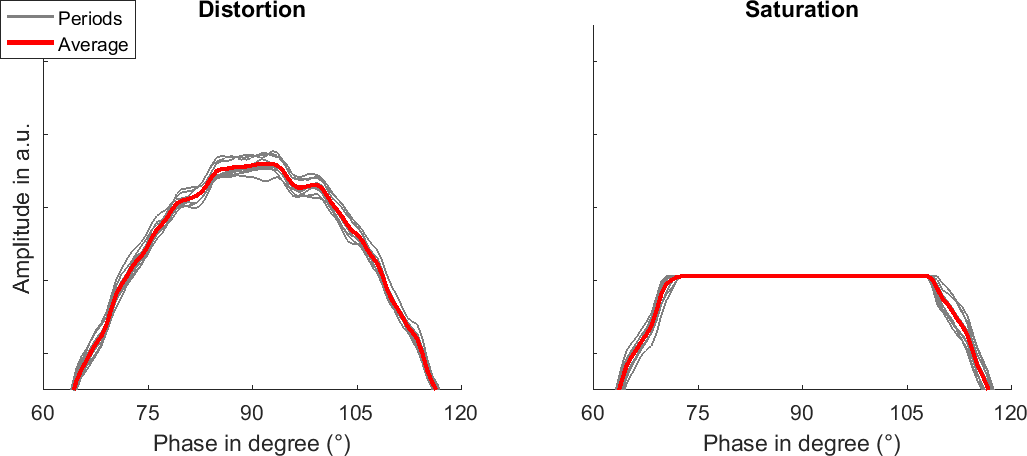
\includegraphics[width=\textwidth]{./img/non_sinusoidality.png}
    \caption{Non-Sinusoidality}
    \figleg{It shows the distortion/saturation of the sinus waveform using two exemplary trials of \gls{tacs}-\gls{eeg}. The gray traces indicate nine invididual periods, while the red trace indicates their average. In the left figure, noe the periodic, but non-sinusoidal waveform. In the right figure, note the saturation.}\label{fig:nonsinus}
\end{figure}

Ideally, the stimulation artifect resembles a sinusoid. Yet, practical experience suggests that the signal is usually distorted to various degrees.~\figref{fig:nonsinus}.

A major reason for distortion by amplifier saturation, i.e.\ the stimulation artifact exhibits an amplitude to large for the dynamic range of the amplifier, causing the signal to be cut off. Even when close to the saturation threshold, non-linearites in the amplifier slew rate can distort the shape. Additionally, the temporally and spatially uneven impedance distribution has been suggested to cause distortion, rendering the resulting waveform periodic, but non-sinusoidal.

\subsection{Computational Demands}

Methods based on adaptive template construction and \gls{tpca}~\citep{Niazy_2005} have been explored for removal of  non-stationary and misshaped \gls{tacs} artifacts~\citep{Helfrich_2014}.  Consider that the process of template construction, the estimation of accurate weights for initial removal and the removal of residual artifacts using  \gls{tpca}  artifact removal is computationally cumbersome, and often requires off-line analysis supported by visual inspection.
This multi-staged template-approach has therefore of limited utility for on-line artifact removal. Furthermore, a critical evaluation has suggested that the residual artifact spans several principal components, and a sufficient artifact removal is not possible with \gls{tpca} \citep{Noury_2016}.

\subsection{Rationale}

We were interested in development of a computationally fast approach, feasible for online artifact removal. At the same time, the approach was required to account for the non-stationarity of the artifacts amplitude, and the possibility of non-sinusoidal distortion and saturation. Ideally, the approach should allow to estimate physiological signals at the frequency of stimulation, even if physiological oscillations were phase-locked to the stimulation signal.

\section{Methods}

\section{Evaluation}

\section{Conclusion}


\bibliographystyle{apalike-oadoi}
\bibliography{sample}

\end{document}
